% !TEX encoding = UTF-8
% !TEX TS-program = pdflatex
% !TEX root = ../tesi.tex

%**************************************************************
\chapter{Architettura per il Context}
\label{cap:architettura-context}
%**************************************************************

L'ultimo step di evoluzione del progetto \textit{Stargate} consiste nell'astrazione \textbf{da stato applicativo a Context}, ovvero contesto di esecuzione dei componenti UI. Sebbene difatti lo stato applicativo rappresenti nella maggioranza dei casi tutto ciò di cui un widget ha bisogno da parte dell'applicazione principale, in alcuni casi è necessario poter accedere anche ad altri oggetti ed addirittura richiamare metodi dalla finestra padre. \\

Si supponga difatti che il widget mappa utilizzi un'istanza \gls{singleton} della classe \texttt{GoogleMaps}, responsabile dei calcoli geografici attraverso le API di Google Maps e condivisa a molteplici componenti UI oltre alla mappa.

In questo caso, il widget mappa ha dunque bisogno del seguente "contesto" per poter correttamente funzionare anche al di fuori della pagina principale: \\

\begin{lstlisting}
interface MapContext {
  googleMaps: GoogleMaps
  state: State
}
\end{lstlisting}

Si può notare come il precedente stato applicativo \texttt{State}, sia ora una delle proprietà del \textit{Context} della mappa e sicuramente la più importante. Tuttavia il passaggio da stato applicativo ad un concetto più generale di "contesto", permette anche l'aggiunta all'interfaccia di un campo per l'istanza singleton di \texttt{GoogleMaps}, senza dover inserire questi nello stato applicativo di cui non fa parte logicamente. 

A livello di architettura fortunatamente vi è poco da modificare, in quanto si tratta solamente di ampliare il concetto di stato applicativo a \textit{Context} e quindi di rinominare i termini. Si parla quindi di \textbf{Context e DerivedContext} invece che \textit{State e DerivedState}.

\begin{figure}[H] 
  \centering 
  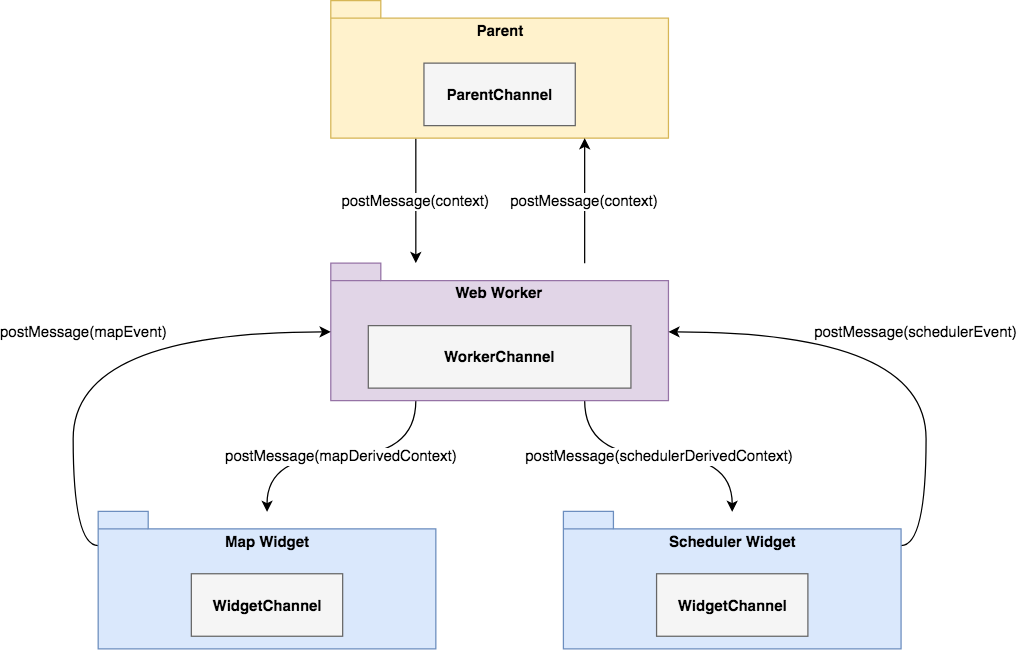
\includegraphics[width=1\columnwidth]{architettura3} 
  \caption{Architettura per il Context}
\end{figure}

\section{Remote Procedure Call (RPC)}

L'introduzione del \textit{Context} porta alla luce una nuova sfida: chiamate di metodi nella finestra padre da parte di widgets. Lo \textit{State} è infatti un'insieme di dati di sola lettura, ma l'istanza \texttt{GoogleMaps} viene invece utilizzata richiamandone metodi con passaggio di parametri e valori di ritorno attesi. \\

Tuttavia l'applicazione principale, il \textit{Web Worker} ed i widget non hanno alcuna condivisione di memoria per cui apparentemente sembrerebbe impossibile per una finestra figlia richiamare un metodo di un oggetto esistente solo nel padre. Nel caso di istanze singleton come \textit{GoogleMaps} non è possibile che ogni widget abbia la sua copia dell'oggetto, poiché violerebbe proprio la definizione di singleton. \\

In questi casi è necessario utilizzare \textbf{Remote Procedure Call (RPC)}, ovvero chiamate chiamate di procedure che avvengono in uno spazio di memoria diverso (solitamente un altro dispositivo della rete), ma in maniera trasparente come normali chiamate locali a procedure/metodi. È desiderabile infatti che il chiamante del \textit{metodo RPC} non conosca i dettagli implementativi della chiamata remota sottostante.

In Java vi è un'implementazione delle chiamate RPC attraverso le \textit{Remote method invocations (RMI)}. \\

Nel caso del progetto \textit{Stargate}, quando il widget esegue una chiamata di un metodo del \textit{Context}, ad esempio \texttt{context.googleMaps.getDistance(a, b)}, in realtà succede il seguente:

\begin{enumerate}
  \item Viene creato un messaggio contenente informazioni sulla chiamata, quali la proprietà del \textit{Context}, il nome del metodo ed i parametri;
  \item Il messaggio viene inviato al \textit{Web Worker};
  \item Il messaggio viene ritrasmesso al \textit{ParentChannel};
  \item Viene invocato l'effettivo metodo nella finestra padre, passando i parametri provenienti dal widget;
  \item Viene generato un messaggio contenente le informazioni della chiamata con l'eventuale valore di ritorno;
  \item Il messaggio di risposta viene inviato al \textit{Web Worker} e ritrasmesso al \textit{WidgetChannel};
  \item Il chiamante riceve il valore di ritorno e può proseguire con il resto della procedura
\end{enumerate}

Per ovvi motivi di performance, una volta chiamato il metodo, la finestra widget mette in pausa la procedura asincrona e prosegue con altre attività evitando di rimanere bloccata in attesa della risposta. L'inconveniente è difatti che tutte le chiamate di metodi nel \textit{Context} diventano asincrone, anche qualora fossero originariamente sincrone.

\begin{figure}[H] 
  \centering 
  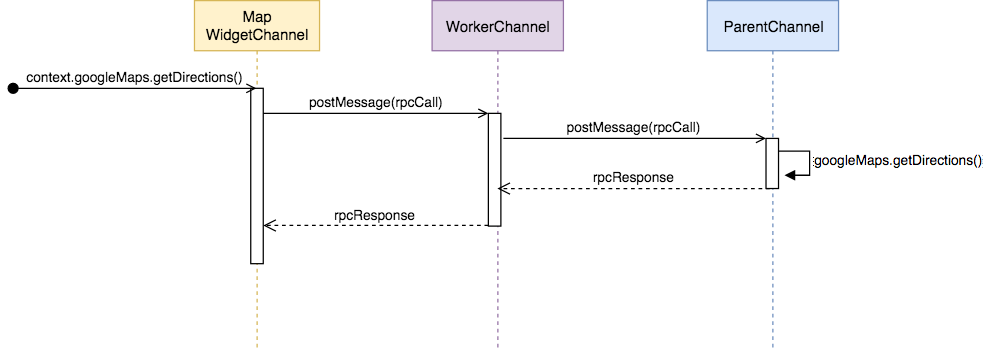
\includegraphics[width=1\columnwidth]{rpc} 
  \caption{Sequenza per una chiamata RPC del context}
\end{figure}


\subsection{Implementazione RPC tramite Proxy}

Bla bla bla
